\documentclass[11pt,a4paper]{report}

\usepackage[english]{babel}
\usepackage[T1]{fontenc}
\usepackage[a4paper,top=3cm,bottom=3cm,left=2cm,right=2.5cm]{geometry}
\usepackage{mathpazo}
\linespread{1.3}
\usepackage{parskip}
\usepackage{titlesec}
\usepackage{caption}
\usepackage{ragged2e}
\AtBeginDocument{\RaggedRight}
\usepackage{graphicx}
\usepackage{array}
\usepackage{tabularray}
\usepackage{enumitem}
\UseTblrLibrary{booktabs}
\usepackage{fancyhdr}
\usepackage{lastpage}
\usepackage[nodayofweek]{datetime}
\usepackage{nth}
\usepackage{graphicx}
\usepackage[hidelinks]{hyperref}

\titleformat{\chapter}[hang]
      {\normalfont\normalsize\bfseries}
      {\thechapter}{1em}{}
\titlespacing*{\chapter}{0pt}{0pt}{1em}
\titleformat{\section}[hang]
      {\normalfont\normalsize\bfseries}
      {\thesection}{1em}{}
\captionsetup{font=normalsize}

\newlist{frsequence}{enumerate}{1}
\SetLabelAlign{center}{\hfil#1\hfil}
\setlist[frsequence]{leftmargin=4.5em,labelwidth=4em,labelsep=0.5em,align=center}

\shortdate
\setcounter{tocdepth}{2}

\pagestyle{fancy}
\fancyhf{}
\fancyhead[L]{Group 7}
\fancyhead[C]{Analysis}
\fancyhead[R]{\today}
\fancyfoot[L]{\nth{1} Semester}
\fancyfoot[R]{\thepage\ / \pageref{LastPage}}
\setlength{\headheight}{14pt}

\fancypagestyle{plain}{
      \fancyhf{}
      \fancyhead[L]{Group 7}
      \fancyhead[C]{Analysis}
      \fancyhead[R]{\today}
      \fancyfoot[L]{\nth{1} Semester}
      \fancyfoot[R]{\thepage\ / \pageref{LastPage}}
}

\title{Game Library Collection System}
\date{\today}

\begin{document}

\begin{titlepage}
      \begin{center}
            \vspace*{0cm}

            \hrule
            \vspace{.5cm}
            {\normalsize \bfseries Analysis 1 \\ Game Library Collection System\\}
            \vspace{.5cm}
            \hrule

            \vspace{1cm}
            Aniara Lyn Inso Lauron: 371989 \\
            Mokhtar Buyema: 370687\\
            Mykyta Lykholobov: 372837\\
            Oleksandr Zavhorodnii: 370951\\
            Sarika Jaman Sonom: 373435

            \par\vspace{0.8cm}
            
\includegraphics[width=0.8\textwidth]{vialogo.jpg}\par

            \vspace{0.7cm}
            {\normalsize Software Engineering, 1st Semester\\}

            \vspace{0.3cm}
            {\normalsize Via University College\\ Horsens, Denmark\\}

            \vspace{1cm}
            {\normalsize \today}
      \end{center}
\end{titlepage}

\tableofcontents

\chapter{Introduction}

\section{Analysis}

As players accumulate titles over time, managing a growing game collection
can become increasingly difficult. This localized, single-user library
management system addresses that problem by providing an isolated data
environment centered on the individual gamer. The application restricts
data modifications to the user's personal catalog.

The process of managing the catalog has four primary parts:
\begin{enumerate}
      \item \textbf{Add:} The gamer can manually add a game title to their
            collection, including its title, genre, and description.
      \item \textbf{Edit:} The gamer can update a saved game's title, genre,
            and description to keep the catalog up to date.
      \item \textbf{Locate:} The gamer can search or filter for one or more
            games. Results are sorted alphabetically to make browsing easier.
      \item \textbf{Remove:} The gamer can delete a game from their collection.
\end{enumerate}

\section{Scope}

The system is limited to catalog management. Installing, launching, or
executing games is outside its scope.

This application is a foundation for a larger system that may eventually
include user connectivity. The design should allow for possible online
features or community modules in the future. The current iteration focuses
on making the four core catalog operations intuitive and reliable.

\chapter{Requirements}

\section{Functional Requirements}

\begin{enumerate}
      \item \textbf{Managing games in one place.}
            As a gamer, I want to add games to my collection so that I can keep
            information about all my games in one place instead of relying on
            memory, notes, or different gaming platforms.

      \item \textbf{Storing game information.}
            As a gamer, I want to store information about each game, such as its
            title, genre, platform, completion status, favorite status, and playtime
            so that I can maintain a complete overview of my collection.

      \item \textbf{Finding specific games.}
            As a gamer, I want to search for games using different criteria, such as
            title, genre, or favorite status, so that I can quickly find the games
            I am looking for.

      \item \textbf{Browsing games by genre.}
            As a gamer, I want to filter games by genre so that I can easily find
            games that match my interests and preferences.

      \item \textbf{Tracking game progress.}
            As a gamer, I want to update a game's completion status so that I can
            track whether it is completed, currently in progress, or not started.

      \item \textbf{Managing favorite games.}
            As a gamer, I want to mark games as favorites so that I can easily
            identify and access the games I enjoy the most.

      \item \textbf{Viewing favorite games.}
            As a gamer, I want to view only my favorite games so that I can quickly
            find the games I play most often.

      \item \textbf{Updating game information.}
            As a gamer, I want to edit game information so that outdated or
            incorrect information can be corrected whenever necessary.

      \item \textbf{Removing games.}
            As a gamer, I want to remove games from my collection so that it
            remains organized and contains only relevant games.

      \item \textbf{Recording playtime.}
            As a gamer, I want to record the amount of time spent playing each game
            so that I can monitor my gaming activity and better understand my
            gaming habits.

      \item \textbf{Viewing playtime information.}
            As a gamer, I want to view the playtime of my games so that I can
            identify which games I spend the most time playing.

      \item \textbf{Sorting games.}
            As a gamer, I want to sort games using different criteria so that I can
            organize and browse my collection more efficiently.

      \item \textbf{Saving the collection.}
            As a gamer, I want the system to save my game collection so that my
            information is not lost when the application is closed.

      \item \textbf{Loading saved information.}
            As a gamer, I want previously saved game information to load when the
            application starts so that I can continue using the system without
            entering the information again.
\end{enumerate}

\section{Non-Functional Requirements}

\begin{enumerate}
      \setcounter{enumi}{14}

      \item \textbf{Performance and latency.}
            Sorting, filtering, and searching through a collection of up to
            1,000 games must display results within 0.5 seconds to maintain a fast
            and responsive application.

      \item \textbf{Usability and default behavior.}
            The system must sort games alphabetically by default, allowing the user
            to scan and evaluate their backlog at a glance.

      \item \textbf{Reliability and data integrity.}
            The system must safely persist the user's catalog to local storage.
            In the event of a sudden system crash or power outage, the existing
            library files must not become corrupted.
\end{enumerate}

\section{Use-case Diagram}
\begin{figure}[htbp]
      \centering
      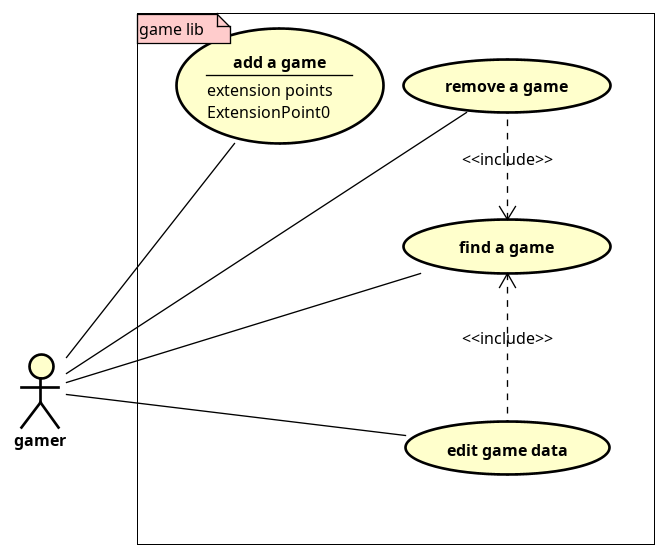
\includegraphics[width=0.75\textwidth]{diagram.png}
      \caption{Use-case diagram for the game library collection system.}
      \label{fig:use-case-diagram}
\end{figure}

\clearpage
\section{Use-case Description}

\begin{longtblr}[
      caption = {Use-case description: Add a game.},
      label = {tab:add-game-use-case}
      ]{
      colspec = {|Q[l,wd=0.27\textwidth]|Q[l,wd=0.65\textwidth]|},
      rowhead = 1,
      hlines,
      vlines
      }
      \textbf{Use-case field} & \textbf{Description}                                                                                                    \\

      Use case                & \textbf{UC-01} Add a game                                                                                                        \\
      Summary                 & Allows the gamer to add a new game to their collection.                                                                 \\
      Actor                   & Gamer                                                                                                                   \\
      Precondition            &
      The game library is open and running.\par
      The gamer has access to their personal game database collection.                                                                                  \\
      Postcondition           & A new game has been added to the library.                                                                               \\
      Base sequence           &
      \begin{frsequence}
            \setlength{\itemsep}{5pt}
            \setlength{\parskip}{5pt}
            \setlength{\parsep}{5pt}
            \item [\textbf{[FR-01]}] The gamer selects ``Add Game''.
            \item [\textbf{[FR-02]}] The system displays a blank form.
            \item [\textbf{[FR-03]}] The gamer enters the game details into the form.
            \item [\textbf{[FR-04]}] The gamer submits the details.
            \item [\textbf{[FR-05]}] The system validates the entered data.
            \item [\textbf{[FR-06]}] The system saves the new game data to the database collection after successful validation.
            \item [\textbf{[FR-07]}] The system displays a success confirmation message and adds
            \item [\textbf{[FR-08]}] The system updates the library catalog view.
      \end{frsequence} \\
      Branch sequence         &
      \textit{Alternative during steps 2--3 of the base sequence, while the
            blank form is open:}
      \begin{frsequence}
            \setlength{\itemsep}{0pt}
            \setlength{\parskip}{0pt}
            \setlength{\parsep}{0pt}
            \item[\textbf{[FR-09]}] The gamer closes the form or selects ``Cancel''.
            \item[\textbf{[FR-10]}] The system discards any text entered into the form fields.
            \item[\textbf{[FR-11]}] The system returns the gamer to the main library catalog view.
            \item[\textbf{[FR-12]}] The system shall not create a new game entry when the form is closed or canceled.
            \item[\textbf{[FR-13]}] The use case ends.
      \end{frsequence}                                          \\
      Exception sequence      &
      \textit{Technical crash during steps 1--3 of the base sequence:}
      \begin{frsequence}
            \setlength{\itemsep}{0pt}
            \setlength{\parskip}{0pt}
            \setlength{\parsep}{0pt}
            \item[\textbf{[FR-14]}] The system encounters a technical error or terminates unexpectedly before saving.
            \item[\textbf{[FR-15]}] The system discards the uncommitted game data.
            \item[\textbf{[FR-16]}] The system shall prevent an unsuccessful save operation from creating an incomplete entry.
            \item[\textbf{[FR-17]}] The postconditions cannot be realized.
      \end{frsequence}                                 \\
      Sub-use case            & None                                                                                                                    \\
      Note                    & Game data may include title, platform, genre, and release year.                                                         \\
\end{longtblr}

\begin{longtblr}[
      caption = {Use-case description: Edit game data.},
      label = {tab:edit-game-use-case}
      ]{
      colspec = {|Q[l,wd=0.27\textwidth]|Q[l,wd=0.65\textwidth]|},
      rowhead = 1,
      hlines,
      vlines
      }
      \textbf{Use-case field} & \textbf{Description}                                                                           \\

      \textbf{Use case}                & \textbf{[UC-02]} Edit game data                                                                         \\
      Summary                 & Allows the gamer to modify saved game details, such as the
      title and genre, to update the game catalog.                                                                             \\
      Actor                   & Gamer                                                                                          \\
      Precondition            &
      The gamer is part of the game library system.\par
      The game information already exists in the user's database collection.                                                   \\
      Postcondition           &
      The updated game information is saved to the system and displayed to
      the gamer.                                                                                                               \\
      Base sequence           &
      \begin{frsequence}
            \setlength{\itemsep}{0pt}
            \setlength{\parskip}{0pt}
            \setlength{\parsep}{0pt}
            \item[\textbf{[FR-18]}] The gamer selects ``Edit Game''.
            \item[\textbf{[FR-19]}] The system displays a form with the current game details.
            \item[\textbf{[FR-20]}] The gamer modifies the information in the form.
            \item[\textbf{[FR-21]}] The gamer selects ``Save''.
            \item[\textbf{[FR-22]}] The system validates the newly entered information.
            \item[\textbf{[FR-23]}] The system updates the database with the new information.
            \item[\textbf{[FR-24]}] The system displays a confirmation message and shows the updated game information in the catalog.
      \end{frsequence} \\
      Branch sequence         &
      \textit{Alternative during steps 1--3 of the base sequence:}
      \begin{frsequence}
            \setlength{\itemsep}{0pt}
            \setlength{\parskip}{0pt}
            \setlength{\parsep}{0pt}
            \item[\textbf{[FR-25]}] The gamer selects ``Cancel''.
            \item[\textbf{[FR-26]}] The system discards the inputs.
            \item[\textbf{[FR-27]}] The system displays the original game details without
                  making changes.
            \item[\textbf{[FR-28]}] The use case ends.
      \end{frsequence}                                             \\
      Exception sequence      &
      \textit{Technical error during steps 1--5 of the base sequence:}
      \begin{frsequence}
            \setlength{\itemsep}{0pt}
            \setlength{\parskip}{0pt}
            \setlength{\parsep}{0pt}
            \item[\textbf{[FR-29]}] The system terminates the session or edit state.
            \item[\textbf{[FR-30]}] The system discards the unsaved form data and newly entered
                  details.
            \item[\textbf{[FR-31]}] The system aborts the database transaction, leaving the
                  original game information unchanged.
            \item[\textbf{[FR-32]}] The postconditions cannot be realized, and the use case ends.
      \end{frsequence}                                     \\
      Sub-use case            & Find a game                                                                                    \\
      Note                    & If the game library was accidentally closed due to technical issues,
      the new information will be saved in local storage and the gamer will be able to continue editing                        \\
\end{longtblr}

\begin{longtblr}[
      caption = {Use-case description: Find a game.},
      label = {tab:find-game-use-case}
      ]{
      colspec = {|Q[l,wd=0.27\textwidth]|Q[l,wd=0.65\textwidth]|},
      rowhead = 1,
      hlines,
      vlines
      }
      \textbf{Use-case field} & \textbf{Description}                                                                           \\

      \textbf{Use case}                & \textbf{[UC-03]} Find a game                                                                            \\
      Summary                 & The gamer locates one or more games in their library by
      searching or filtering.                                                                                                  \\
      Actor                   & Gamer                                                                                          \\
      Precondition            &
      \begin{enumerate}
            \setlength{\itemsep}{0pt}
            \setlength{\parskip}{0pt}
            \setlength{\parsep}{0pt}
            \item The game library application is running.
            \item The library contains at least one game.
      \end{enumerate}                                                                            \\
      Postcondition           & Matching games are displayed, and the gamer can select
      one to view details, edit, or remove.                                                                                    \\
      Base sequence           &
      \begin{frsequence}
            \setlength{\itemsep}{0pt}
            \setlength{\parskip}{0pt}
            \setlength{\parsep}{0pt}
            \item[\textbf{[FR-33]}] The gamer selects the ``Find a game'' button.
            \item[\textbf{[FR-34]}] The system displays a search field and filter options for
                  title, genre, and platform.
            \item[\textbf{[FR-35]}] The gamer enters a search term and/or selects filters.
            \item[\textbf{[FR-36]}] The system searches the library for matching games.
            \item[\textbf{[FR-37]}] The system displays a list of matching games.
            \item[\textbf{[FR-38]}] The gamer selects a game from the list.
            \item[\textbf{[FR-39]}] The system displays the selected game's details.
      \end{frsequence}                                         \\
      Branch sequence         &
      \begin{frsequence}
            \setlength{\itemsep}{0pt}
            \setlength{\parskip}{0pt}
            \setlength{\parsep}{0pt}
            \item[\textbf{[FR-40]}] 3a. The gamer submits an empty search; the system displays
                  all games in the library.
            \item[\textbf{[FR-41]}] 5a. No matching games are found; the system displays
                  ``No games found'' and returns to step 3.
            \item[\textbf{[FR-42]}] 5b. Too many results are found; the gamer adds more filters and returns to step 3.
            \item[\textbf{[FR-43]}] 6a. The gamer cancels the search; the use case ends without a selection.
      \end{frsequence}                \\
      Exception sequence      &
      \begin{frsequence}
            \setlength{\itemsep}{0pt}
            \setlength{\parskip}{0pt}
            \setlength{\parsep}{0pt}
            \item[\textbf{[FR-42]}] 4a.The library data cannot be loaded; the system displays an error message and the use case ends.
      \end{frsequence} \\
      Sub-use case            & None                                                                                           \\
      Note                    & ``Find a game'' is included by ``Remove a game'' and
      ``Edit game data'', since the gamer must locate a game before removing
      or editing it.                                                                                                           \\
\end{longtblr}

\begin{longtblr}[
      caption = {Use-case description: Remove a game.},
      label = {tab:remove-game-use-case}
      ]{
      colspec = {|Q[l,wd=0.27\textwidth]|Q[l,wd=0.65\textwidth]|},
      rowhead = 1,
      hlines,
      vlines
      }
      \textbf{Use-case field} & \textbf{Description}                                                     \\

      \textbf{Use case}                & \textbf{[UC-04]} Remove a game                                                    \\
      Summary                 & Allows the gamer to remove a game from their collection.                 \\
      Actor                   & Gamer                                                                    \\
      Precondition            &
      The gamer is logged into the game library system.\par
      The library catalog contains at least one saved game in the user's
      database collection.                                                                               \\
      Postcondition           &
      The selected game record is permanently removed from the database and
      is no longer visible in the library catalog.                                                       \\
      Base sequence           &
      \begin{frsequence}
            \setlength{\itemsep}{0pt}
            \setlength{\parskip}{0pt}
            \setlength{\parsep}{0pt}
            \item[\textbf{[FR-44]}] The gamer selects ``Find a Game''.
            \item[\textbf{[FR-45]}] The system displays the search bar or game list.
            \item[\textbf{[FR-46]}] The gamer selects the game they want to remove.
            \item[\textbf{[FR-47]}] The system displays the selected game's details and a ``Delete'' button.
            \item[\textbf{[FR-48]}] The gamer selects ``Delete''.
            \item[\textbf{[FR-49]}] The system displays a confirmation prompt asking,
                  ``Are you sure you want to delete this game?''
            \item[\textbf{[FR-50]}] The gamer selects ``Confirm''.
            \item[\textbf{[FR-51]}] The system removes the game data from the user's database
                  collection.
            \item[\textbf{[FR-52]}] The system displays a success message and updates the library catalog view.
      \end{frsequence} \\
      Branch sequence         &
      \textit{Alternative at step 6 of the base sequence, while the
            confirmation prompt is displayed:}
      \begin{frsequence}
            \setlength{\itemsep}{0pt}
            \setlength{\parskip}{0pt}
            \setlength{\parsep}{0pt}
            \item[\textbf{[FR-53]}] The gamer selects ``Cancel'' or ``No''.
            \item[\textbf{[FR-54]}] The system closes the prompt without changing the database.
            \item[\textbf{[FR-55]}] The system returns the gamer to the game details page.
            \item[\textbf{[FR-56]}] The game record remains in the library catalog.
            \item[\textbf{[FR-57]}] The use case ends.
      \end{frsequence}                 \\
      Exception sequence      &
      \textit{Error while the system attempts to remove the data:}
      \begin{frsequence}
            \setlength{\itemsep}{0pt}
            \setlength{\parskip}{0pt}
            \setlength{\parsep}{0pt}
            \item[\textbf{[FR-58]}] The system encounters a database or technical error while
                  removing the game.
            \item[\textbf{[FR-59]}] The system displays an error message stating that the game
                  could not be removed.
            \item[\textbf{[FR-60]}] The system aborts the deletion and rolls back any partial
                  changes.
            \item[\textbf{[FR-61]}] The game record remains in the user's collection.
            \item[\textbf{[FR-62]}] The success postconditions cannot be realized, and the use
                  case ends.
      \end{frsequence}                  \\
      Sub-use case            & Find a game                                                              \\
      Note                    & The application asks for confirmation before removing a game.            \\
\end{longtblr}



\end{document}
